\documentclass{article}
\usepackage{amsmath,amsthm,amssymb} % Required for math stuff
\usepackage{graphicx} % Required for inserting images
\usepackage{tikz} % Required for drawing graphs

\newtheorem{theorem}{Theorem}[section]

\title{Project 3}
\author{Mengxiang Jiang}
\date{\today}



\begin{document}

\maketitle

\section{Introduction}
When I was taking chemistry in high school, I learned about structural 
isomers. These were molecules that had the same chemical formula, but 
different structures.
The example given was that of butane ($C_4H_{10}$), which can
either be a straight chain of 4 carbon atoms, 
or a branched chain with 3 carbon atoms in a row and one carbon atom 
attached to the middle carbon atom (see Figure 1).
\begin{figure}[ht!]
\centering
% Standard article (10pt) friendly sizing
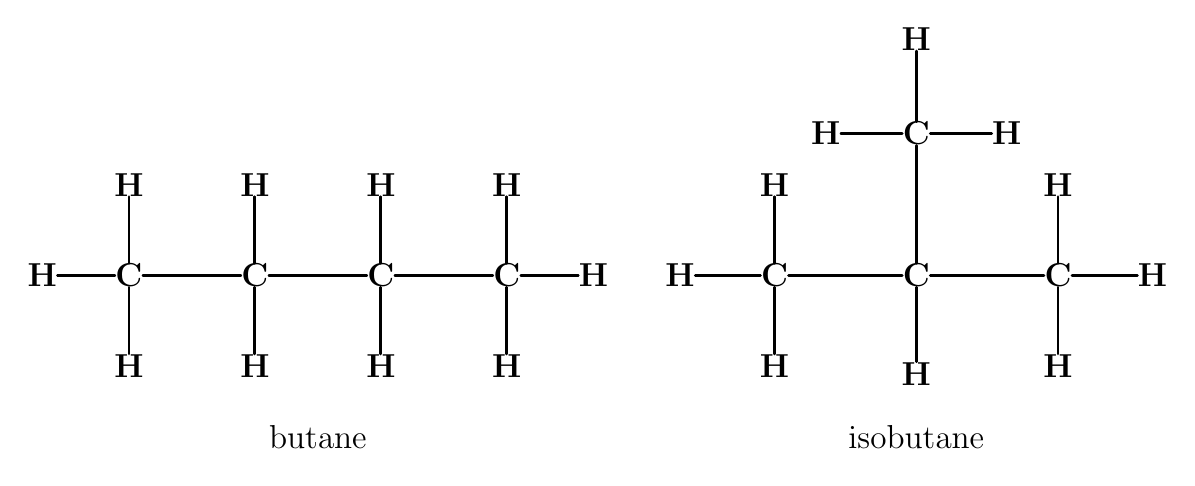
\begin{tikzpicture}[
  bond/.style={line width=1.0pt, line cap=round},
  atom/.style={inner sep=0pt, font=\large\bfseries},
  lab/.style={font=\large}
]

% ===================== n-Butane =====================
    \begin{scope}[xshift=0cm,yshift=0cm]
    % Carbons
    \node[atom] (C1) at (0,0)   {C};
    \node[atom] (C2) at (1.6,0) {C};
    \node[atom] (C3) at (3.2,0) {C};
    \node[atom] (C4) at (4.8,0) {C};

    % C-C bonds
    \draw[bond] (C1)--(C2)--(C3)--(C4);

    % Hydrogens
    \node[atom] (H1L) at (-1.1,0) {H}; \draw[bond] (H1L)--(C1);
    \node[atom] (H1U) at (0,1.15)  {H}; \draw[bond] (H1U)--(C1);
    \node[atom] (H1D) at (0,-1.15) {H}; \draw[bond] (H1D)--(C1);

    \node[atom] (H2U) at (1.6,1.15)  {H}; \draw[bond] (H2U)--(C2);
    \node[atom] (H2D) at (1.6,-1.15) {H}; \draw[bond] (H2D)--(C2);

    \node[atom] (H3U) at (3.2,1.15)  {H}; \draw[bond] (H3U)--(C3);
    \node[atom] (H3D) at (3.2,-1.15) {H}; \draw[bond] (H3D)--(C3);

    \node[atom] (H4R) at (5.9,0) {H}; \draw[bond] (H4R)--(C4);
    \node[atom] (H4U) at (4.8,1.15)  {H}; \draw[bond] (H4U)--(C4);
    \node[atom] (H4D) at (4.8,-1.15) {H}; \draw[bond] (H4D)--(C4);

    % Label
    \node[lab] at (2.4,-2.05) {butane};
    \end{scope}

    % ===================== Isobutane =====================
    \begin{scope}[xshift=10.0cm,yshift=0cm]
    % Carbons
    \node[atom] (Cc) at (0,0)   {C};   % central
    \node[atom] (Cl) at (-1.8,0){C};   % left
    \node[atom] (Cr) at (1.8,0) {C};   % right
    \node[atom] (Ct) at (0,1.8) {C};   % top

    % C-C bonds
    \draw[bond] (Cl)--(Cc)--(Cr);
    \draw[bond] (Ct)--(Cc);

    % Central H
    \node[atom] (HcD) at (0,-1.25) {H}; \draw[bond] (HcD)--(Cc);

    % Left methyl Hs
    \node[atom] (HlL) at (-3.0,0) {H}; \draw[bond] (HlL)--(Cl);
    \node[atom] (HlU) at (-1.8,1.15) {H}; \draw[bond] (HlU)--(Cl);
    \node[atom] (HlD) at (-1.8,-1.15){H}; \draw[bond] (HlD)--(Cl);

    % Right methyl Hs
    \node[atom] (HrR) at (3.0,0) {H}; \draw[bond] (HrR)--(Cr);
    \node[atom] (HrU) at (1.8,1.15) {H}; \draw[bond] (HrU)--(Cr);
    \node[atom] (HrD) at (1.8,-1.15){H}; \draw[bond] (HrD)--(Cr);

    % Top methyl Hs
    \node[atom] (HtU) at (0,3.0) {H}; \draw[bond] (HtU)--(Ct);
    \node[atom] (HtL) at (-1.15,1.8){H}; \draw[bond] (HtL)--(Ct);
    \node[atom] (HtR) at (1.15,1.8) {H}; \draw[bond] (HtR)--(Ct);

    % Label
    \node[lab] at (0,-2.05) {isobutane};
    \end{scope}

\end{tikzpicture}
\caption{The two structural isomers of $C_4H_{10}$.}
\end{figure}
Butane belongs to a class of molecules called alkanes, which are composed entirely of carbon and hydrogen atoms
with only single bonds. Alkanes can have many structural isomers depending on the
number of carbon atoms present in the molecule.
The number grows very rapidly as you can see from the table in Figure 2.
\begin{figure}[ht!]
\centering
\begin{tabular}{|c|c|}
\hline
Number of Carbons & Number of Structural Isomers \\
\hline
1 & 1 \\
2 & 1 \\
3 & 1 \\
4 & 2 \\
5 & 3 \\
6 & 5 \\
7 & 9 \\
8 & 18 \\
9 & 35 \\
10 & 75 \\
\hline
\end{tabular}
\caption{Number of structural isomers of alkanes with different number of carbon atoms.}
\end{figure}
This made me wonder: is there a formula or algorithm that can determine the number of structural isomers for any given alkane? After doing some research, I found out about the Online Encyclopedia of Integer Sequences (OEIS) which has a sequence (A000602) that lists the number of structural isomers for alkanes. It presents a generating function by Eric Rains and Neil Sloane based on Arthur Cayley's work in 1875 \cite{rains1999cayley}.

\section{The Generating Function}
First we will give a few definitions.
\begin{itemize}
    \item A \textbf{graph} is a collection of vertices (or nodes) connected by edges.
    \item The \textbf{degree} of a node is the number of edges connected to it.
    \item The \textbf{valence} of a graph is the maximum degree of any node in the graph. In our case, since carbon atoms can form up to 4 bonds, we will be considering graphs that are 4-valent.
    \item A \textbf{tree} is a connected graph with no cycles. This means there is exactly one path between any two nodes in the tree.
    \item A \textbf{rooted tree} is a tree with one vertex designated as the root, giving the tree a sense of direction away from the root.
    \item The \textbf{diameter} of a tree is the length of the longest path between any two nodes in the tree.
    \item The \textbf{center} of a tree is the node (or pair of nodes) that is in the middle of the longest path in the tree.
\end{itemize}


\begin{section}{Bibliography}
    \bibliographystyle{plain}
    \bibliography{refs}
\end{section}

\end{document}
